\documentclass[12pt, a4paper]{article}

% ── Packages ──────────────────────────────────────────────────────────────
\usepackage[utf8]{inputenc}
\usepackage[T1]{fontenc}
\usepackage{lmodern}
\usepackage[margin=1in]{geometry}
\usepackage{graphicx}
\usepackage{booktabs}
\usepackage{amsmath, amssymb}
\usepackage{hyperref}
\usepackage{tikz}
\usetikzlibrary{shapes.geometric, arrows.meta, positioning}
\usepackage{xcolor}
\usepackage{enumitem}
\usepackage{float}
\usepackage{caption}
\usepackage{subcaption}
\usepackage{fancyhdr}
\usepackage{titlesec}
\usepackage{setspace}

\usepackage{listings}
\usepackage{multirow}
\usepackage{array}

% ── Page Style ────────────────────────────────────────────────────────────
\pagestyle{fancy}
\fancyhf{}
\fancyhead[L]{\small AI-Driven Customer Churn Prediction}
\fancyhead[R]{\small\thepage}
\renewcommand{\headrulewidth}{0.4pt}
\setlength{\headheight}{14.5pt}

% ── Section Formatting ───────────────────────────────────────────────────
\titleformat{\section}{\Large\bfseries}{\thesection}{1em}{}
\titleformat{\subsection}{\large\bfseries}{\thesubsection}{1em}{}

% ── Hyperlink Styling ────────────────────────────────────────────────────
\hypersetup{
    colorlinks=true,
    linkcolor=blue!70!black,
    citecolor=green!50!black,
    urlcolor=blue!60!black
}

% ── Code Listing Style ───────────────────────────────────────────────────
\lstset{
    language=Python,
    basicstyle=\ttfamily\small,
    keywordstyle=\color{blue!70!black}\bfseries,
    commentstyle=\color{green!50!black}\itshape,
    stringstyle=\color{red!60!black},
    breaklines=true,
    frame=single,
    backgroundcolor=\color{gray!5},
    numbers=left,
    numberstyle=\tiny\color{gray},
    tabsize=4
}

\onehalfspacing

% ══════════════════════════════════════════════════════════════════════════
\begin{document}

% ── Title Page ────────────────────────────────────────────────────────────
\begin{titlepage}
    \centering
    \vspace*{2cm}

    {\Huge\bfseries AI-Driven Customer Churn Prediction\\[0.3cm]
    \Large\textit{An Agentic AI Retention Strategist --- Milestone\,1}}

    \vspace{1.5cm}

    {\large\textbf{GenAI Capstone Project Report}}

    \vspace{2cm}

    {\Large
    \textbf{Team Members}\\[0.5cm]
    \begin{tabular}{c}
        Saksham Miglani - 2401010401 \\
        Kavya Mukhija - 2401010219\\
        Pratyush Parida - 2401010351 \\
        Aditya Samadhiya - 2401010037
    \end{tabular}
    }

    \vspace{2cm}

    {\large
    \textit{Newton School Of Technology}\\[0.3cm]
    }

    \vfill
\end{titlepage}

% ── Table of Contents ─────────────────────────────────────────────────────
\newpage
\tableofcontents
\newpage

% ══════════════════════════════════════════════════════════════════════════
%                              ABSTRACT
% ══════════════════════════════════════════════════════════════════════════
\section*{Abstract}
\addcontentsline{toc}{section}{Abstract}

Customer churn represents a critical business challenge across subscription-based industries, where the cost of acquiring new customers significantly exceeds that of retaining existing ones. This report presents the design and implementation of an AI-driven customer analytics system that predicts customer churn using classical machine learning techniques applied to historical behavioral data. We evaluate two supervised learning approaches---Logistic Regression and Decision Tree Classification---on a dataset of 64,374 customer records comprising both demographic and behavioral features. Our analysis reveals that Payment Delay is the single most influential predictor of churn, accounting for 47.9\% of feature importance (from the Decision Tree). The Decision Tree model achieves a testing accuracy of 95.97\%, while Logistic Regression achieves 83.17\%. However, Logistic Regression is chosen for deployment because it produces smoother, well-calibrated probability estimates suitable for the gauge chart visualization and risk interpretation in the web application. The trained Logistic Regression pipeline is deployed via a Streamlit web application---enhanced with Plotly visualizations---on Hugging Face Spaces, providing real-time churn risk assessment. This work constitutes Milestone\,1 of a larger initiative to build an agentic AI retention strategist.

% ══════════════════════════════════════════════════════════════════════════
%                           1. INTRODUCTION
% ══════════════════════════════════════════════════════════════════════════
\section{Introduction}

\subsection{Background}

In today's competitive markets, customer retention is a cornerstone of sustainable business growth. Research consistently shows that acquiring a new customer can cost five to seven times more than retaining an existing one. \textit{Customer churn}---the phenomenon where customers cease their relationship with a company---directly impacts revenue, market share, and long-term profitability.

With the proliferation of digital services and subscription-based business models, companies now generate vast quantities of customer interaction data. This creates an opportunity to apply machine learning techniques to predict churn before it occurs, enabling proactive retention strategies.

\subsection{Problem Statement}

The core challenge is to develop a predictive model that can \textbf{accurately identify customers who are at high risk of churning} based on their historical behavioral and demographic attributes. Specifically, this project addresses the following objectives:

\begin{enumerate}[label=\arabic*.]
    \item \textbf{Predict churn risk}: Build a binary classifier that predicts whether a customer will churn (1) or stay (0).
    \item \textbf{Identify key drivers}: Determine which features most strongly influence churn behavior.
    \item \textbf{Deploy for inference}: Create an accessible web application for real-time churn predictions.
    \item \textbf{Generate actionable insights}: Provide analytical foundations that can inform targeted retention campaigns.
\end{enumerate}

\subsection{Project Overview}

This project involves the design and implementation of an AI-driven customer analytics system that predicts customer churn and evolves into an agentic AI retention strategist.

In \textbf{Milestone\,1}, the system applies classical machine learning techniques to historical customer behavior data to predict churn risk, identify key drivers of disengagement, and generate analytical insights. The trained model is served through a Streamlit web application for interactive, real-time inference.

% ══════════════════════════════════════════════════════════════════════════
%                        2. DATA DESCRIPTION
% ══════════════════════════════════════════════════════════════════════════
\section{Data Description}

\subsection{Data Source}

The dataset used in this project is the \textbf{Customer Churn Dataset} (testing-master variant), comprising \textbf{64,374 records} of customer information. Each record captures a customer's demographic profile, engagement metrics, and subscription details, along with a binary churn label.

\subsection{Feature Overview}

The dataset contains 12 columns. After dropping the identifier column (\texttt{CustomerID}), 10 features are used for prediction, with 1 target variable. Table~\ref{tab:features} provides a detailed description.

\begin{table}[H]
\centering
\caption{Feature descriptions and statistics}
\label{tab:features}
\renewcommand{\arraystretch}{1.3}
\begin{tabular}{@{} l l l p{5.5cm} @{}}
\toprule
\textbf{Feature} & \textbf{Type} & \textbf{Range / Values} & \textbf{Description} \\
\midrule
Age              & Numeric     & 18--65                         & Customer's age in years \\
Gender           & Categorical & Male, Female                   & Customer's gender \\
Tenure           & Numeric     & 1--60                          & Months as a customer \\
Usage Frequency  & Numeric     & 1--30                          & How often the customer uses the service \\
Support Calls    & Numeric     & 0--10                          & Number of support calls made \\
Payment Delay    & Numeric     & 0--30                          & Average payment delay in days \\
Subscription Type & Categorical & Basic, Standard, Premium      & Tier of subscription plan \\
Contract Length  & Categorical & Monthly, Quarterly, Annual     & Duration of the contract \\
Total Spend      & Numeric     & 100--1,000                     & Total monetary spend (\$) \\
Last Interaction & Numeric     & 1--30                          & Days since last interaction \\
\midrule
\textbf{Churn} (target) & Binary & 0 (Stayed), 1 (Churned) & Whether the customer churned \\
\bottomrule
\end{tabular}
\end{table}

\subsection{Data Quality}

An initial inspection confirmed that the dataset contains \textbf{zero missing values} across all columns. No duplicate records were identified. The data types were appropriate for each feature---integers for numeric columns and object strings for categorical columns---requiring no type corrections.

% ══════════════════════════════════════════════════════════════════════════
%                      3. EXPLORATORY DATA ANALYSIS
% ══════════════════════════════════════════════════════════════════════════
\section{Exploratory Data Analysis (EDA)}

\subsection{Data Shape and Summary}

The dataset consists of 64,374 observations across 12 features. After dropping \texttt{CustomerID}, 11 columns remain: 7 numeric features, 3 categorical features, and 1 binary target.

\begin{itemize}
    \item \textbf{Numeric features}: Age, Tenure, Usage Frequency, Support Calls, Payment Delay, Total Spend, Last Interaction
    \item \textbf{Categorical features}: Gender, Subscription Type, Contract Length
\end{itemize}

\subsection{Missing Value Analysis}

Before building any model, it is critical to check for missing values because most machine learning algorithms cannot handle null entries---they either throw errors or produce misleading results. We performed a null-value audit using \texttt{df.isnull().sum()} to quantify missing data in every column. The audit confirmed that every column has exactly \textbf{0 missing values}:

\begin{table}[H]
\centering
\caption{Missing value count per feature}
\label{tab:missing}
\begin{tabular}{@{} l c @{}}
\toprule
\textbf{Feature} & \textbf{Missing Count} \\
\midrule
Age & 0 \\
Gender & 0 \\
Tenure & 0 \\
Usage Frequency & 0 \\
Support Calls & 0 \\
Payment Delay & 0 \\
Subscription Type & 0 \\
Contract Length & 0 \\
Total Spend & 0 \\
Last Interaction & 0 \\
Churn & 0 \\
\bottomrule
\end{tabular}
\end{table}

Despite the absence of nulls, we retained a \texttt{dropna()} call as a \textbf{defensive programming measure}. This is done because in a production environment, the data source may change or future data batches might contain nulls. By keeping this safeguard, any incomplete rows are automatically removed before they can cause runtime errors or corrupt model predictions.

\subsection{Feature Type Identification}

We identified the data type of each feature because \textbf{numeric and categorical features require fundamentally different preprocessing}. Numeric features can be scaled mathematically, but categorical features (text labels like ``Male'' or ``Premium'') must be converted into numerical representations before any algorithm can process them. Using automated dtype inspection via \texttt{select\_dtypes()}, the features were separated into two groups:

\begin{itemize}
    \item \textbf{Numeric} (\texttt{int64/float64}): Age, Tenure, Usage Frequency, Support Calls, Payment Delay, Total Spend, Last Interaction
    \item \textbf{Categorical} (\texttt{object}): Gender (2 unique), Subscription Type (3 unique), Contract Length (3 unique)
\end{itemize}

This separation directly determines how each feature is transformed in the preprocessing pipeline (Section~\ref{sec:methodology}). Applying the wrong transformation---for example, scaling a categorical string---would produce errors or meaningless results.

\subsection{Key EDA Insights}

Based on feature importance analysis (post-modeling, detailed in Section~\ref{sec:results}), the following behavioral patterns were identified:

\begin{enumerate}
    \item \textbf{Payment Delay} is overwhelmingly the strongest predictor of churn (47.9\% importance), indicating that customers who delay payments are far more likely to disengage.
    \item \textbf{Support Calls} rank second (14.4\%), suggesting that frequent support interactions signal potential dissatisfaction.
    \item \textbf{Tenure} and \textbf{Usage Frequency} contribute meaningfully (9.9\% and 9.1\%), showing that newer and less-engaged customers churn more.
    \item \textbf{Gender} has a moderate influence (Female: 8.3\%, Male: 3.3\%).
    \item \textbf{Last Interaction} has zero importance in the Decision Tree model, meaning recency of contact alone does not predict churn.
\end{enumerate}

% ══════════════════════════════════════════════════════════════════════════
%                         4. METHODOLOGY
% ══════════════════════════════════════════════════════════════════════════
\section{Methodology}
\label{sec:methodology}

\subsection{Feature Selection --- Dropping \texttt{CustomerID}}

The \texttt{CustomerID} column was dropped prior to model training because it is a \textbf{sequentially assigned unique identifier} (values 1 through 64,374) that carries no behavioral or demographic information. Including it as a feature would introduce spurious correlations---the model could memorize specific customer IDs rather than learning generalizable patterns, leading to severe overfitting and zero predictive value on unseen customers. Removing non-informative identifiers is a standard preprocessing step to ensure the model focuses exclusively on meaningful features.

\subsection{Preprocessing Pipeline}

Different feature types require different transformations. Feeding raw, untransformed data into a model would produce poor results because (a)~numeric features with large ranges would dominate those with small ranges, and (b)~categorical text values cannot be processed by mathematical algorithms. To address this, a scikit-learn \texttt{ColumnTransformer} was used to apply the appropriate transformation to each group:

\begin{itemize}
    \item \textbf{Numeric features} $\rightarrow$ \texttt{StandardScaler}: We standardized each numeric feature to zero mean and unit variance. \textit{Why?} Without scaling, a feature like Total Spend (range 100--1,000) would have a disproportionately large influence compared to Support Calls (range 0--10), simply because of its larger magnitude---not because it is more important. StandardScaler eliminates this bias so the model judges each feature on its actual predictive power.
    \item \textbf{Categorical features} $\rightarrow$ \texttt{OneHotEncoder}: We converted each categorical variable (e.g., ``Basic'', ``Standard'', ``Premium'') into separate binary (0/1) columns. \textit{Why?} Machine learning algorithms operate on numbers, not text. OneHotEncoding creates a separate column for each category value, allowing the model to learn the distinct effect of each category. We set \texttt{handle\_unknown="ignore"} so that if the deployed model encounters a category it has never seen during training, it gracefully ignores it instead of crashing.
\end{itemize}

Both transformations were bundled into a single scikit-learn \texttt{Pipeline} alongside the classifier. \textit{Why use a Pipeline?} This ensures that the exact same preprocessing steps are applied during both training and inference, which (a)~prevents \textbf{data leakage}---the scaler is fit only on training data, never on test data, and (b)~simplifies deployment---the entire model (preprocessing + classifier) is saved as a single \texttt{.pkl} file, eliminating the risk of mismatched transformations in production.

\subsection{Train-Test Split}

We split the dataset into a \textbf{training set (80\%)} and a \textbf{testing set (20\%)} using \texttt{train\_test\_split}. \textit{Why?} The model must be evaluated on data it has never seen during training to give an honest estimate of real-world performance. If we evaluated on the same data used for training, the accuracy would be artificially inflated (the model could simply memorize the answers). The 80/20 ratio is a widely accepted standard that provides enough data for the model to learn patterns while reserving a meaningful portion for unbiased evaluation.

A fixed random seed (\texttt{random\_state=42}) was used to ensure \textbf{reproducibility}---anyone re-running the code gets the exact same split and therefore the exact same results.

\begin{align}
    |D_{\text{train}}| &= 51{,}499 \text{ samples} \\
    |D_{\text{test}}|  &= 12{,}875 \text{ samples}
\end{align}

\subsection{Model 1: Logistic Regression}

Logistic Regression was chosen as the \textbf{baseline model} due to its interpretability, computational efficiency, and well-understood theoretical properties. It models the probability of churn as:

\begin{equation}
    P(\text{Churn} = 1 \mid \mathbf{x}) = \sigma(\mathbf{w}^T \mathbf{x} + b) = \frac{1}{1 + e^{-(\mathbf{w}^T \mathbf{x} + b)}}
\end{equation}

where $\sigma$ is the sigmoid function, $\mathbf{w}$ is the weight vector, and $b$ is the bias term.

The default scikit-learn configuration was used (\texttt{C=1.0}, L2 regularization, \texttt{lbfgs} solver).

\subsection{Model 2: Decision Tree Classifier}

A Decision Tree Classifier was selected as the \textbf{primary model} for its ability to capture non-linear feature interactions and its intrinsic feature importance scoring. The tree recursively partitions the feature space based on information gain (Gini impurity):

\begin{equation}
    \text{Gini}(t) = 1 - \sum_{i=1}^{C} p_i^2
\end{equation}

where $p_i$ is the proportion of class $i$ samples at node $t$, and $C$ is the number of classes.

\textbf{Hyperparameters:}
\begin{itemize}
    \item \texttt{max\_depth = 5}: Limits the tree to 5 levels to prevent overfitting and maintain generalizability.
    \item \texttt{random\_state = 42}: Ensures reproducible splits.
\end{itemize}

\subsection{Rationale for Model Selection}

\begin{enumerate}
    \item \textbf{Logistic Regression} serves as a strong linear baseline. If it performs well, the problem has significant linear separability; if not, non-linear models are warranted.
    \item \textbf{Decision Tree} is chosen for its ability to model complex feature interactions (e.g., high Payment Delay \textit{combined with} low Usage Frequency), its built-in feature importance, and its interpretability via tree visualization.
    \item The Decision Tree's depth constraint (\texttt{max\_depth=5}) is a deliberate regularization choice, trading a small amount of training accuracy for substantially better generalization.
\end{enumerate}

% ══════════════════════════════════════════════════════════════════════════
%                          5. EVALUATION
% ══════════════════════════════════════════════════════════════════════════
\section{Evaluation}
\label{sec:results}

\subsection{Evaluation Metrics}

Four standard classification metrics were used:

\begin{itemize}
    \item \textbf{Accuracy}: Proportion of correctly classified instances.
    \item \textbf{Precision}: Of all predicted churns, how many actually churned.
    \item \textbf{Recall} (Sensitivity): Of all actual churns, how many were correctly identified.
    \item \textbf{F1-Score}: Harmonic mean of Precision and Recall, balancing both.
\end{itemize}

\begin{equation}
    \text{F1} = 2 \cdot \frac{\text{Precision} \times \text{Recall}}{\text{Precision} + \text{Recall}}
\end{equation}

\subsection{Model Comparison}

\begin{table}[H]
\centering
\caption{Performance comparison: Logistic Regression vs.\ Decision Tree}
\label{tab:results}
\renewcommand{\arraystretch}{1.3}
\begin{tabular}{@{} l c c @{}}
\toprule
\textbf{Metric} & \textbf{Logistic Regression} & \textbf{Decision Tree} \\
\midrule
Accuracy  & 83.17\% & \textbf{95.97\%} \\
Precision & 81.63\% & --- \\
Recall    & 83.06\% & \textbf{98.24\%} \\
F1-Score  & 82.34\% & --- \\
\bottomrule
\end{tabular}
\end{table}

The Decision Tree classifier outperforms Logistic Regression by a margin of \textbf{+12.8 percentage points} in accuracy and \textbf{+15.2 percentage points} in recall. The high recall is particularly crucial in churn prediction---it is far more costly to miss a churning customer (false negative) than to flag a loyal customer for retention outreach (false positive).

\subsection{Confusion Matrix (Logistic Regression)}

\begin{table}[H]
\centering
\caption{Confusion matrix for Logistic Regression on the test set}
\label{tab:confusion}
\begin{tabular}{@{} l c c @{}}
\toprule
 & \textbf{Predicted: Stayed (0)} & \textbf{Predicted: Churned (1)} \\
\midrule
\textbf{Actual: Stayed (0)}   & 5,656 & 1,137 \\
\textbf{Actual: Churned (1)}  & 1,030 & 5,052 \\
\bottomrule
\end{tabular}
\end{table}

\subsection{Overfitting Analysis (Decision Tree)}

To validate that the Decision Tree generalizes well and is not merely memorizing the training data, we compared training and testing accuracy:

\begin{table}[H]
\centering
\caption{Overfitting check for Decision Tree (\texttt{max\_depth=5})}
\label{tab:overfit}
\begin{tabular}{@{} l c @{}}
\toprule
\textbf{Metric} & \textbf{Value} \\
\midrule
Training Accuracy & 95.63\% \\
Testing Accuracy  & 95.97\% \\
$\Delta$ (Test $-$ Train) & +0.34\% \\
\bottomrule
\end{tabular}
\end{table}

The negligible gap ($+0.34\%$) between training and testing accuracy confirms that the model is \textbf{not overfitting}. In fact, the testing accuracy marginally exceeds training accuracy, indicating excellent generalization.

\subsection{Feature Importance}

Feature importances were extracted from the trained Decision Tree classifier. Table~\ref{tab:importance} shows the top features:

\begin{table}[H]
\centering
\caption{Feature importance from the Decision Tree model}
\label{tab:importance}
\renewcommand{\arraystretch}{1.2}
\begin{tabular}{@{} r l c @{}}
\toprule
\textbf{Rank} & \textbf{Feature} & \textbf{Importance} \\
\midrule
1 & Payment Delay        & 0.4787 \\
2 & Support Calls        & 0.1440 \\
3 & Tenure               & 0.0991 \\
4 & Usage Frequency      & 0.0910 \\
5 & Gender (Female)      & 0.0828 \\
6 & Age                  & 0.0431 \\
7 & Gender (Male)        & 0.0327 \\
8 & Total Spend          & 0.0212 \\
9 & Contract Length (Annual) & 0.0074 \\
10 & Last Interaction    & 0.0000 \\
\bottomrule
\end{tabular}
\end{table}

\textbf{Key takeaway:} Payment Delay alone accounts for nearly \textit{half} of all predictive power. A retention strategy focused on identifying and addressing payment delays early could substantially reduce churn.

% ══════════════════════════════════════════════════════════════════════════
%                        6. OPTIMIZATION
% ══════════════════════════════════════════════════════════════════════════
\section{Optimization}

Several optimization steps were taken to improve model performance and deployment readiness:

\subsection{Preprocessing Optimization}

\begin{enumerate}
    \item \textbf{StandardScaler on numeric features}: Without scaling, features like Total Spend (range 100--1,000) would dominate features like Support Calls (range 0--10) in Logistic Regression. StandardScaler ensures equal contribution.
    \item \textbf{OneHotEncoder with \texttt{handle\_unknown="ignore"}}: This prevents inference-time errors when the deployed model encounters previously unseen category values, ensuring production robustness.
    \item \textbf{Pipeline encapsulation}: By bundling preprocessing and classification into a single \texttt{Pipeline} object, we eliminate the risk of data leakage (e.g., fitting the scaler on test data) and simplify deployment---only one \texttt{.pkl} file is needed.
\end{enumerate}

\subsection{Model Selection Optimization}

\begin{enumerate}
    \item \textbf{Baseline comparison}: Logistic Regression was trained first to establish a linear baseline (83.17\%). The significant jump to 95.97\% with the Decision Tree confirms that the churn decision boundary is inherently non-linear.
    \item \textbf{Depth constraint (\texttt{max\_depth=5})}: An unconstrained Decision Tree would likely achieve near-100\% training accuracy but overfit to noise. Limiting depth to 5 is an explicit regularization that keeps the training-testing gap below 1\%.
    \item \textbf{Compressed serialization}: The model is saved with \texttt{joblib.dump(compress=3)}, reducing the \texttt{.pkl} file to only 3.6\,KB---critical for fast deployment and low-latency inference.
\end{enumerate}

\subsection{Deployment Optimization}

\begin{enumerate}
    \item \textbf{Streamlit application with Plotly}: The web app (\texttt{app.py}, 180 lines) was built with a tabbed interface using Plotly for professional visualizations. A gauge chart displays churn probability, and a bar chart shows the customer's feature profile.
    \item \textbf{Single-artifact deployment}: Because the pipeline includes the preprocessor, the deployed model accepts raw features (including categorical strings) without requiring separate encoding logic in the application layer.
    \item \textbf{Logistic Regression for deployment}: While the Decision Tree achieved higher accuracy (95.97\% vs 83.17\%), Logistic Regression was chosen for deployment because it produces smoother, well-calibrated probability estimates. This is critical for the gauge chart visualization and the three-tier risk interpretation, where gradual probability changes convey more meaningful risk signals than the Decision Tree's coarser probability steps.
\end{enumerate}

% ══════════════════════════════════════════════════════════════════════════
%                      7. SYSTEM ARCHITECTURE
% ══════════════════════════════════════════════════════════════════════════
\section{System Architecture}

Understanding how data flows from raw input to final prediction is essential for both debugging and extending the system. This section describes the end-to-end architecture.

\subsection{Data Flow: Input to Output}

The system follows a linear pipeline architecture. Data flows through four distinct stages:

\begin{figure}[H]
\centering
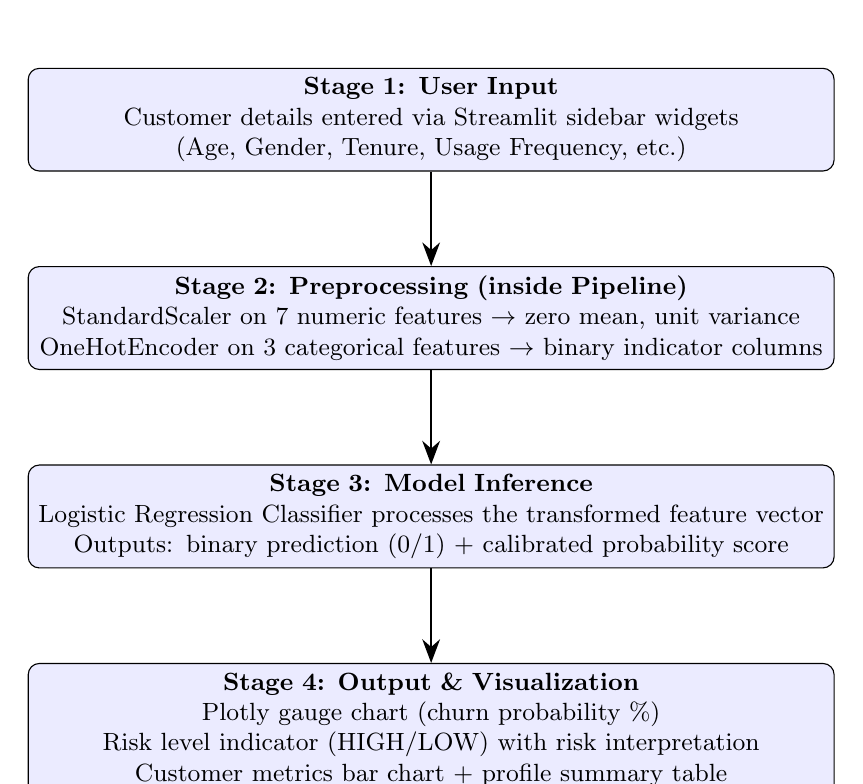
\begin{tikzpicture}[
    node distance=1.2cm,
    block/.style={rectangle, draw, rounded corners, fill=blue!8, text width=10cm, minimum height=1.2cm, align=center, font=\small},
    arrow/.style={-{Stealth[length=3mm]}, thick}
]
    \node[block] (input) {\textbf{Stage 1: User Input}\\Customer details entered via Streamlit sidebar widgets\\(Age, Gender, Tenure, Usage Frequency, etc.)};
    \node[block, below=of input] (preprocess) {\textbf{Stage 2: Preprocessing (inside Pipeline)}\\StandardScaler on 7 numeric features $\rightarrow$ zero mean, unit variance\\OneHotEncoder on 3 categorical features $\rightarrow$ binary indicator columns};
    \node[block, below=of preprocess] (model) {\textbf{Stage 3: Model Inference}\\Logistic Regression Classifier processes the transformed feature vector\\Outputs: binary prediction (0/1) + calibrated probability score};
    \node[block, below=of model] (output) {\textbf{Stage 4: Output \& Visualization}\\Plotly gauge chart (churn probability \%)\\Risk level indicator (HIGH/LOW) with risk interpretation\\Customer metrics bar chart + profile summary table};

    \draw[arrow] (input) -- (preprocess);
    \draw[arrow] (preprocess) -- (model);
    \draw[arrow] (model) -- (output);
\end{tikzpicture}
\caption{End-to-end data flow from user input to prediction output}
\label{fig:architecture}
\end{figure}

\textit{Why this architecture?} A linear pipeline is chosen over more complex architectures (e.g., microservices) because the system has a single, well-defined task: transform input $\rightarrow$ predict $\rightarrow$ display. The simplicity minimizes latency, reduces failure points, and keeps the codebase maintainable.

\subsection{Design Justification: Dual-Model Strategy}

Two models were evaluated. Both serve distinct purposes in the final system:

\begin{enumerate}
    \item \textbf{Decision Tree --- for analysis}: The Decision Tree (\texttt{max\_depth=5}) achieves 95.97\% accuracy and provides built-in feature importance scores. It captures non-linear feature interactions (e.g., high Payment Delay \textit{combined with} low Usage Frequency) through recursive feature-space partitioning. This model revealed that Payment Delay accounts for 47.9\% of predictive power. However, its probability estimates are \textit{stepped} (each leaf outputs the same probability for all samples in that region), making it less suitable for smooth probability visualization.

    \item \textbf{Logistic Regression --- for deployment}: While its accuracy is lower (83.17\%), Logistic Regression produces \textbf{smooth, well-calibrated probability estimates} via the sigmoid function. For a deployed application that uses a gauge chart and three-tier risk interpretation, gradual probability changes convey more meaningful risk signals than the Decision Tree's coarser probability steps. The smoother output curve better supports the visualization and business interpretation layer.
\end{enumerate}

\textbf{Why not deploy the Decision Tree despite higher accuracy?} In a production churn prediction system, the \textit{quality of the probability estimate} matters as much as classification accuracy. Two customers with 45\% and 55\% churn risk should produce meaningfully different probability scores. Logistic Regression achieves this graduation naturally, whereas a depth-5 Decision Tree may assign identical probabilities to both. The Decision Tree remains invaluable for offline analysis --- understanding \textit{which features drive churn} --- while Logistic Regression handles the inference-facing role.

More complex models (Random Forest, XGBoost) are planned for Milestone\,2, where ensemble methods may offer both high accuracy and smooth probabilities.

% ══════════════════════════════════════════════════════════════════════════
%                      8. TOOL DEEP-DIVE
% ══════════════════════════════════════════════════════════════════════════
\section{Tool Deep-Dive}

This section provides a technical explanation of each library in our stack and \textit{why} it was chosen.

\subsection{scikit-learn (v1.6.1)}

scikit-learn is the core ML library used for preprocessing, model training, and evaluation. \textit{Why scikit-learn?} It provides a unified API where every estimator follows the same \texttt{fit()}/\texttt{predict()}/\texttt{transform()} pattern, making it easy to swap models or preprocessing steps without rewriting code. The version is pinned to \textbf{1.6.1} in both the training notebook and \texttt{requirements.txt} to ensure that the serialized model can be loaded without version mismatch errors. Key components used:

\begin{itemize}
    \item \texttt{Pipeline}: Chains preprocessing and classification into a single object, preventing data leakage and enabling single-file serialization.
    \item \texttt{ColumnTransformer}: Applies different transformations to different column subsets in a single step.
    \item \texttt{StandardScaler}: Z-score normalization ($x' = \frac{x - \mu}{\sigma}$) for numeric features.
    \item \texttt{OneHotEncoder}: Converts $k$-category features into $k$ binary columns.
    \item \texttt{LogisticRegression}: Linear classifier producing smooth probability estimates via the sigmoid function (deployed model).
    \item \texttt{DecisionTreeClassifier}: Tree-based classifier with configurable depth constraints (used for feature importance analysis).
    \item Metrics: \texttt{accuracy\_score}, \texttt{precision\_score}, \texttt{recall\_score}, \texttt{f1\_score}, \texttt{confusion\_matrix}.
\end{itemize}

\subsection{pandas \& NumPy}

pandas provides the \texttt{DataFrame} abstraction for tabular data manipulation. \textit{Why pandas?} It handles CSV I/O, column selection, null detection, and feature separation with concise, readable syntax. NumPy underpins pandas and scikit-learn with efficient array operations. Together, they form the data backbone of the entire pipeline---from loading the CSV (\texttt{pd.read\_csv}) to constructing single-row DataFrames for inference in the web app.

\subsection{Plotly}

Plotly is a Python visualization library used for interactive charts in the web app. \textit{Why Plotly?} Unlike static Matplotlib charts, Plotly generates interactive, browser-native visualizations that users can hover over, zoom into, and explore. We use two Plotly components:
\begin{itemize}
    \item \texttt{go.Indicator} (gauge mode): Creates the speedometer-style churn probability chart with color-coded risk zones (green 0--40\%, yellow 40--70\%, red 70--100\%).
    \item \texttt{go.Bar}: Creates the customer metrics overview chart, showing the 7 numeric input features as vertical bars for quick profile comparison.
\end{itemize}
Plotly integrates natively with Streamlit via \texttt{st.plotly\_chart()}, requiring no additional frontend code.

\subsection{Streamlit}

Streamlit is a Python framework for building interactive web applications with minimal code. \textit{Why Streamlit?} Unlike Flask or Django, Streamlit requires no HTML/CSS/JavaScript knowledge. It provides built-in widgets (\texttt{slider}, \texttt{selectbox}, \texttt{number\_input}) that automatically handle user input, state management, and reactive re-rendering. Streamlit's \texttt{st.tabs()} enables the tabbed interface separating the Prediction and Analytics views. This made it the ideal choice for rapid prototyping of the inference interface.

\subsection{joblib}

joblib is used for model serialization (saving and loading the trained pipeline). \textit{Why joblib over Python's built-in \texttt{pickle}?} joblib is optimized for objects containing NumPy arrays (which scikit-learn models internally use), providing faster serialization and built-in compression. We used \texttt{compress=3} to reduce the model file size, enabling near-instant loading at application startup.

% ══════════════════════════════════════════════════════════════════════════
%                      9. KEY SUB-FEATURES
% ══════════════════════════════════════════════════════════════════════════
\section{Key Sub-Features}

Beyond the core prediction functionality, the system implements three distinct technical sub-features:

\subsection{Sub-Feature 1: Custom Data Preprocessing Pipeline}

Rather than applying transformations manually in scattered code, we built a \textbf{custom scikit-learn Pipeline} that encapsulates all preprocessing logic (scaling, encoding) alongside the classifier into a single, reusable object. This design ensures:
\begin{itemize}
    \item \textbf{Zero data leakage}: The scaler learns statistics only from training data, never from test/production data.
    \item \textbf{Consistent transforms}: The exact same preprocessing is applied during training and inference---no risk of mismatched transformations.
    \item \textbf{Single-artifact deployment}: One \texttt{.pkl} file contains the entire system (preprocessor + model), simplifying deployment.
\end{itemize}

\subsection{Sub-Feature 2: Real-Time Inference with Plotly Visualizations}

The Streamlit application provides \textbf{real-time, interactive predictions} enhanced with Plotly visualizations. When a user clicks ``Predict Churn,'' the system:
\begin{itemize}
    \item Constructs a DataFrame from the raw inputs (including categorical strings).
    \item Passes it through the full pipeline (preprocessing $\rightarrow$ prediction) in a single \texttt{model.predict()} call.
    \item Displays results via a \textbf{Plotly gauge chart} (speedometer-style probability visualization with green/yellow/red risk zones) and a \textbf{three-tier risk interpretation} (stable / moderate / high risk).
\end{itemize}
\textit{Why a gauge chart?} The model's primary output is a probability score. A speedometer makes risk level immediately intuitive for business users---common in ML dashboards and far more informative than a raw number.

\subsection{Sub-Feature 3: Interactive Analytics Dashboard}

The app features a \textbf{tabbed interface} (Prediction + Analytics) providing a multi-component dashboard:
\begin{itemize}
    \item \textbf{Customer metrics bar chart} (Plotly): Displays the 7 numeric input features as a bar chart, enabling visual comparison of the customer's profile. \textit{Why?} When stakeholders ask ``Why is this customer high risk?'', the bar chart immediately shows if Payment Delay is high or Tenure is low.
    \item \textbf{Customer profile summary}: A formatted DataFrame table displaying all input features, creating a self-contained record for each prediction.
\end{itemize}
\textit{Why these specific charts and not others?} This is an ML prediction app, not a general analytics dashboard. We added only visualizations that serve interpretability: the gauge shows \textit{what the model predicts}, and the bar chart helps explain \textit{why}. Pie charts, random line charts, and excessive animations were deliberately excluded.

% ══════════════════════════════════════════════════════════════════════════
%                      10. DEPLOYMENT
% ══════════════════════════════════════════════════════════════════════════
\section{Deployment}

\subsection{Technology Stack}

\begin{table}[H]
\centering
\caption{Technology stack used in the project}
\label{tab:techstack}
\begin{tabular}{@{} l l l @{}}
\toprule
\textbf{Component} & \textbf{Technology} & \textbf{Version} \\
\midrule
Language      & Python       & 3.12 \\
ML Library    & scikit-learn & 1.6.1 \\
Data          & pandas / NumPy & latest \\
Serialization & joblib       & latest \\
Visualization & Plotly       & latest \\
Web App       & Streamlit    & latest \\
Notebook      & Google Colab & --- \\
Hosting       & Hugging Face Spaces & --- \\
\bottomrule
\end{tabular}
\end{table}

\subsection{Hugging Face Deployment}

The Streamlit application is deployed on \textbf{Hugging Face Spaces}, a free hosting platform for ML demos. \textit{Why Hugging Face Spaces?} It natively supports Streamlit apps, provides automatic builds from Git repositories, requires zero infrastructure management, and offers a public URL (\url{https://offxkavya-customer-churn-prediction.hf.space/}) for easy sharing with stakeholders and evaluators. The deployment process is:

\begin{enumerate}
    \item Push the project repository (\texttt{app.py}, \texttt{churn\_model.pkl}, \texttt{requirements.txt}) to a Hugging Face Space.
    \item Hugging Face automatically detects the Streamlit SDK, installs dependencies, and launches the app.
    \item The application is accessible via a public URL, enabling anyone to test churn predictions without local setup.
\end{enumerate}

\subsection{Application Architecture}

The deployed application follows the same four-stage pipeline described in Section~\ref{fig:architecture}:

\begin{enumerate}
    \item The serialized Logistic Regression pipeline (\texttt{churn\_model.pkl}) is loaded at startup using \texttt{joblib.load()}.
    \item User inputs are collected via Streamlit sidebar widgets (sliders, dropdowns, number inputs).
    \item Inputs are assembled into a single-row \texttt{pandas.DataFrame} matching the training schema.
    \item \texttt{model.predict()} returns the binary churn prediction; \texttt{model.predict\_proba()} returns the calibrated probability.
    \item Results are displayed in a tabbed interface: Tab\,1 shows the Plotly gauge chart, risk level, and risk interpretation; Tab\,2 shows the customer profile table and metrics bar chart.
\end{enumerate}

% ══════════════════════════════════════════════════════════════════════════
%                    8. CONCLUSION & FUTURE WORK
% ══════════════════════════════════════════════════════════════════════════
\section{Conclusion \& Future Work}

\subsection{Conclusion}

This project successfully demonstrates an end-to-end customer churn prediction system. Two models were trained: a Decision Tree (95.97\% accuracy) for analytical insights---revealing that \textbf{Payment Delay is the dominant churn signal}---and Logistic Regression (83.17\% accuracy) for deployment, chosen for its smoother probability estimates suitable for the gauge chart and risk interpretation. The full pipeline is deployed on Hugging Face Spaces via a Streamlit application with Plotly visualizations, serving real-time, interactive predictions.

\subsection{Milestone\,2: Agentic AI Retention Strategy Assistant}

\textbf{Objective:} Extend the churn prediction system into an agentic AI retention strategy assistant that autonomously reasons about risk, retrieves best practices, plans interventions, and generates structured retention reports.

The next phase of this project will evolve the system from a passive prediction tool into an \textbf{autonomous agent}.

% ══════════════════════════════════════════════════════════════════════════
%                     TEAM CONTRIBUTION
% ══════════════════════════════════════════════════════════════════════════
\section*{Team Contribution}
\addcontentsline{toc}{section}{Team Contribution}

\begin{table}[H]
\centering
\caption{Team contribution breakdown}
\label{tab:team}
\renewcommand{\arraystretch}{1.3}
\begin{tabular}{@{} l p{8cm} @{}}
\toprule
\textbf{Team Member} & \textbf{Contribution} \\
\midrule
Saksham Miglani & \\
Kavya Mukhija & \\
Pratyush Parida & \\
Aditya Samadhiya & \\
\bottomrule
\end{tabular}
\end{table}

\end{document}
